% Created 2018-12-08 Sat 15:38
% Intended LaTeX compiler: pdflatex
\documentclass[11pt]{article}
\usepackage[utf8]{inputenc}
\usepackage{lmodern}
\usepackage[T1]{fontenc}
\usepackage{fixltx2e}
\usepackage{graphicx}
\usepackage{longtable}
\usepackage{float}
\usepackage{wrapfig}
\usepackage{rotating}
\usepackage[normalem]{ulem}
\usepackage{amsmath}
\usepackage{textcomp}
\usepackage{marvosym}
\usepackage{wasysym}
\usepackage{amssymb}
\usepackage{amsmath}
\usepackage[theorems, skins]{tcolorbox}
\usepackage[version=3]{mhchem}
\usepackage[numbers,super,sort&compress]{natbib}
\usepackage{natmove}
\usepackage{url}
\usepackage{minted}
\usepackage{underscore}
\usepackage[linktocpage,pdfstartview=FitH,colorlinks,
linkcolor=blue,anchorcolor=blue,
citecolor=blue,filecolor=blue,menucolor=blue,urlcolor=blue]{hyperref}
\usepackage{attachfile}
\date{\today}
\title{}
\begin{document}

\tableofcontents

\section{{\bfseries\sffamily ASSIGNED} exam3-1 uncertainty\hfill{}\textsc{autograd:uncertainty:p1:2:nori}}
\label{sec:org33ba6c0}
\textbf{This is an exam. You must be present in the exam room to get credit for this problem unless you have prior permission from the instructor. You may not talk during the exam except to ask an instructor a question. By turning this in, you agree that this work is your own, and you did not get unauthorized help to complete it or provide unauthorized help to anyone else. You may not modify your exam answer after the due time without permission.}

The time required to reach a particular conversion \(X\) in a reactor is given by this integral equation:

\(t = \int_0^X \frac{1}{k C_{A0} (1 - X)^2} dX\)

In this problem, \(k = 1e-3\) L/mol/min, and \(C_{A0} = 1\) mol/L.

We aim to find the uncertainty in the amount of time required to reach a conversion of 0.9. The uncertainty is estimated by:

\(\sigma_t = \sqrt{\frac{\partial t}{\partial k}^2 \sigma_k^2 + \frac{\partial t}{\partial C_{A0}}^2 \sigma_{C_{A0}}^2 }\)

with \(\sigma_k = 1e-4\) and \(\sigma_{C_{A0}} = 0.01\).

To evaluate those derivatives, we need a differentiable integrator. You can use this implementation of the trapezoid rule for that. You cannot use the quad function.

\begin{minted}[frame=lines,fontsize=\scriptsize,linenos]{ipython}
import autograd.numpy as np

def trapz(y, x):
    d = np.diff(x)
    return np.sum((y[0:-1] + y[1:]) * d / 2)
\end{minted}

First, use the equation above and the provided trapz function to find the time required to reach 90\% conversion for this reactor.

Next, use the formula for \(\sigma_t\) to estimate the uncergtainty in this time.


\subsection{solution\hfill{}\textsc{solution}}
\label{sec:orgf854c59}

\begin{minted}[frame=lines,fontsize=\scriptsize,linenos]{ipython}
import autograd.numpy as np
k = 1e-3
sigma_k = 1e-4

Ca0 = 1.0
sigma_Ca0 = 0.01


X = np.linspace(0.0, 0.9, 5000)

def trapz(y, x):
    d = np.diff(x)
    return np.sum((y[0:-1] + y[1:]) * d / 2)

def t(k, Ca0):
    integrand = 1./(k*Ca0)*(1./(1-X)**2)
    return trapz(integrand, X)

print(t(k, Ca0))
\end{minted}

9000.00539675

\begin{minted}[frame=lines,fontsize=\scriptsize,linenos]{ipython}
dtdk = grad(t, 0)
dtdC = grad(t, 1)

sigma_t = np.sqrt(dtdk(k, Ca0)**2 * sigma_k**2 + dtdC(k, Ca0)**2 * sigma_Ca0**2)
sigma_t
\end{minted}

\begin{verbatim}
904.48881132260317
\end{verbatim}


\section{{\bfseries\sffamily ASSIGNED} exam3-2 eigenvalue\hfill{}\textsc{LA:p2:3:mingjie}}
\label{sec:org2f31744}
\textbf{This is an exam. You must be present in the exam room to get credit for this problem unless you have prior permission from the instructor. You may not talk during the exam except to ask an instructor a question. By turning this in, you agree that this work is your own, and you did not get unauthorized help to complete it or provide unauthorized help to anyone else. You may not modify your exam answer after the due time without permission.}

We have mostly focused on numerical solutions to ODEs. Sometimes, it is possible to leverage Python to obtain analytical solutions though. This problem will focus on a way to do that. We will focus on these equations:

\(y_1'(t) = -0.02 y_1 + 0.02 y_2\)

\(y_2'(t) = 0.02 y_1 - 0.02 y_2\)

with the initial conditions that \(y_1(0) = 0\) and \(y_2(0) = 150\).

We can rewrite the equations in matrix form:

\(\mathbf{y'} = \mathbf{A} \mathbf{y}\)

Here we have \(\mathbf{y'} = \left[\begin{array}{c} y_1'(t) \\ y_2'(t)\end{array}\right]\) and \(\mathbf{y} = \left[\begin{array}{c} y_1(t) \\ y_2(t)\end{array}\right]\). \(\mathbf{A}\) is the array of coefficients.

This is a set of constant coefficient, coupled ODEs. We can try a solution of the form:

\(\mathbf{y} = \mathbf{x} e^{\lambda t}\), where we have an unknown vector \(\mathbf{x}\) and \(\lambda\), and we seek to find values for these that solve the equations.

If you plug this in to the equations then we find:

\(\mathbf{y'} = \lambda \mathbf{x} e^{\lambda t} = \mathbf{A} \mathbf{x} e^{\lambda t}\)

Or, with some minor rearrangement:

\(\mathbf{A} \mathbf{x} = \lambda \mathbf{x}\)

This is an eigenvalue problem, and the solutions to it are the pairs of eigenvalues (\(\lambda\)) and corresponding eigenvectors (\(\mathbf{x}\)).

Find the eigenvalues and eigenvectors of this system of equations:

The solution to the system of ODEs is then a linear combination defined by:

\(\mathbf{y(t)} = c_1 \mathbf{x_1} e^{\lambda_1 t} + c_2 \mathbf{x_2} e^{\lambda_2 t}\)

where \(c_i\) are arbitrary constants, and \(\mathbf{x_i}\) is the i\(^{\text{th}}\) eigenvector that corresponds to the i\(^{\text{th}}\) eigenvalue \(\lambda_i\). To find the values of \(c_i\) we must use the initial conditions. At \(t=0\) we can express this in the form:

\begin{equation}
\left[\begin{array}{c}y_1(0) \\ y_2(0)\end{array}\right]=
[\begin{array}{cc}\mathbf{x_1} & \mathbf{x_2}\end{array}]
\left[\begin{array}{c}c_1\\c_2\end{array}\right]
\end{equation}

where \([\begin{array}{cc}\mathbf{x_1} & \mathbf{x_2}\end{array}]\) is an array with \(\mathbf{x_i}\) in the i\(^{\text{th}}\) column, in other words it is an array of the eigenvectors in column form.

Solve this linear equation for the unknown coefficients \(\mathbf{c}\).

Finally, combine all of this information to get the complete solution

\(\mathbf{y(t)} = c_1 \mathbf{x_1} e^{\lambda_1 t} + c_2 \mathbf{x_2} e^{\lambda_2 t}\). There is not a simple matrix algebra way to do this, so I suggest you do it as:

\(y1(t) = c_1 \mathbf{x_1}[0] e^{\lambda_1 t} + c_2 \mathbf{x_2}[0] e^{\lambda_2 t}\)

and

\(y2(t) = c_1 \mathbf{x_1}[1] e^{\lambda_1 t} + c_2 \mathbf{x_2}[1] e^{\lambda_2 t}\)


and plot the solution for \(y_1(t)\) and \(y_2(t)\) from t=0 to t=100.

\subsection{solution\hfill{}\textsc{solution}}
\label{sec:orgedd7b79}

\begin{minted}[frame=lines,fontsize=\scriptsize,linenos]{ipython}
A = np.array([[-0.02, 0.02],
              [0.02, -0.02]])

evals, evecs = np.linalg.eig(A)

print(evals, evecs)
\end{minted}

[ 0.   -0.04] [[ 0.70710678 -0.70710678]
 [ 0.70710678  0.70710678]]

\begin{minted}[frame=lines,fontsize=\scriptsize,linenos]{ipython}
c = np.linalg.solve(evecs, [0, 150])
c
\end{minted}

\begin{verbatim}
array([ 106.06601718,  106.06601718])
\end{verbatim}

\begin{minted}[frame=lines,fontsize=\scriptsize,linenos]{ipython}
t = np.linspace(0, 100)

x1 = evecs[:, 0]
x2 = evecs[:, 1]

y1 = c[0] * x1[0] * np.exp(evals[0] * t) + c[1] * x2[0] * np.exp(evals[1] * t)
y2 = c[1] * x1[1] * np.exp(evals[0] * t) + c[1] * x2[1] * np.exp(evals[1] * t)

plt.plot(t, y1, t, y2)
\end{minted}

\begin{verbatim}
[<matplotlib.lines.Line2D at 0x1193c9d68>,
 <matplotlib.lines.Line2D at 0x118c65668>]
\end{verbatim}



\begin{center}
\includegraphics[width=.9\linewidth]{obipy-resources/73232f0e737f26c048822a8e09245932-2031mDW.png}
\end{center}


Here is the numpy way of writing this solution. It is more advanced syntax than we have used in class and involves combinations of matrix algebra, elementwise operations and broadcasting.

\begin{minted}[frame=lines,fontsize=\scriptsize,linenos]{ipython}
y = c[None, :] * evecs @ np.array([np.exp(evals[0] * t),
                                   np.exp(evals[1] * t)])
# transpose y so it is in columns.
plt.plot(t, y.T)
\end{minted}

\begin{verbatim}
[<matplotlib.lines.Line2D at 0x11a168d30>,
 <matplotlib.lines.Line2D at 0x11a168f28>]
\end{verbatim}



\begin{center}
\includegraphics[width=.9\linewidth]{obipy-resources/73232f0e737f26c048822a8e09245932-2031ZAE.png}
\end{center}




\section{{\bfseries\sffamily ASSIGNED} exam3-3 nla - continuation\hfill{}\textsc{autograd:ode:p3:3:john}}
\label{sec:org5d6658b}
\textbf{This is an exam. You must be present in the exam room to get credit for this problem unless you have prior permission from the instructor. You may not talk during the exam except to ask an instructor a question. By turning this in, you agree that this work is your own, and you did not get unauthorized help to complete it or provide unauthorized help to anyone else. You may not modify your exam answer after the due time without permission.}

A common problem in solving nonlinear problems is \emph{how to make the initial guess}?

Let's consider finding the solution to the following nonlinear equations:

\(2 + x + y - x^2 + 8 x y + y^3 = 0\)

\(1 + 2x - 3y + x^2 + xy - y e^x = 0\)

The strategy we work on here is to reformulate these equations with a new variable \(\lambda\)

\(2 + x + y + \lambda(- x^2 + 8 x y + y^3) = 0\)

\(1 + 2x - 3y + \lambda(x^2 + xy - y e^x) = 0\)

\subsubsection{Part 1 solve the linear problem}
\label{sec:orgd7996e9}
If \(\lambda=1\) then we have the original nonlinear equations. If you set \(\lambda=0\) though, you have a simple linear set of equations to solve. Find a solution to those equations for \(\lambda=0\):

This solution represents the solution to the equations when \(\lambda=0\). If we could derive a set of equations for \(\frac{dx}{d\lambda}\) and \(\frac{dy}{d\lambda}\), then we can treat this linear solution as an initial value, and integrate the ODEs from \(\lambda=0\) to \(\lambda=1\) to find the solution to the nonlinear equations. In what follows, we motivate how to derive those equations.

\subsubsection{Part 2 formulate a system of ODEs to solve the nonlinear problem}
\label{sec:org4ba9eca}

Next, we consider the equations as

\(f(x, y) = 2 + x + y + \lambda(- x^2 + 8 x y + y^3) = 0\)

\(g(x, y) = 1 + 2x - 3y + \lambda(x^2 + xy - y e^x) = 0\)

from calculus, you can show that:

\(\frac{\partial f}{\partial x}\frac{\partial x}{\partial \lambda}+\frac{\partial f}{\partial y}\frac{\partial y}{\partial \lambda}=-\frac{\partial f}{\partial \lambda}\)

\(\frac{\partial g}{\partial x}\frac{\partial x}{\partial \lambda}+\frac{\partial g}{\partial y}\frac{\partial y}{\partial \lambda}=-\frac{\partial g}{\partial \lambda}\)

You can rewrite this in a linear algebra form as:

\begin{equation}
\left[\begin{array}{cc}
\frac{\partial f}{\partial x} \frac{\partial f}{\partial y} \\
\frac{\partial g}{\partial x} \frac{\partial g}{\partial y}
\end{array}\right]
\left[\begin{array}{c}
\frac{\partial x}{\partial \lambda}\\
\frac{\partial y}{\partial \lambda}
\end{array}\right]
=
\left[\begin{array}{c}
-\frac{\partial f}{\partial \lambda}\\
-\frac{\partial g}{\partial \lambda}
\end{array}\right]
\end{equation}

The matrix on the left is the Jacobian of \(F = [f(x,y), g(x, y)]\). This means you can solve for:

\[\left[\begin{array}{c}
\frac{\partial x}{\partial \lambda}\\
\frac{\partial y}{\partial \lambda}
\end{array}\right]
=
\mathbf{J}^{-1}
\left[\begin{array}{c}
-\frac{\partial f}{\partial \lambda}\\
-\frac{\partial g}{\partial \lambda}
\end{array}\right]\]

This last equation defines a set of differential equations that can be integrated from \(\lambda=0\) where we know what (x, y) are, to \(\lambda=1\) which leads to a solution to the original set of nonlinear equations!

Use the last equation to define a function for a system of ODEs, and then integrate the system of ODES from \(\lambda=0\) to \(\lambda=1\) to find the solution to the nonlinear set of equations. The solution is the value of \(x, y\) at \(\lambda=1\).

\subsubsection{Part 3 Verify the solution you found}
\label{sec:org8cd0081}

Use a method of your choice to verify your solution from Part 2.


\subsection{solution\hfill{}\textsc{solution}}
\label{sec:org0f999b4}

\begin{minted}[frame=lines,fontsize=\scriptsize,linenos]{ipython}
import autograd.numpy as np
from autograd import jacobian

def F(X, L):
    x, y = X
    f = (2.0 + x + y) + L * (-x**2 + 8 * x * y + y**3)
    g = (1.0 + 2.0 * x - 3.0 * y) + L * (x**2 + x * y - y * np.exp(x))
    return np.array([f, g])

J = jacobian(F)
J(np.array([-1.4, -0.6]), 0.0)

dFdL = jacobian(F, 1)

x0 = np.linalg.solve([[1., 1.], [2., -3.]],[ -2, -1])
print(x0)

def ode(X, L):
    x, y = X
    j = J(np.array([x, y]), L)
    dXdL = np.linalg.inv(j) @ -dFdL(np.array([x, y]), L)
    return dXdL

from scipy.integrate import odeint

lambda_span = np.linspace(0, 1, 1000)

X = odeint(ode, x0, lambda_span)

xsol, ysol = X[-1]
print('The solution is at x={0:1.3f}, y={1:1.3f}'.format(xsol, ysol))
print(F([xsol, ysol], 1))
\end{minted}

[-1.4 -0.6]
The solution is at x=-1.000, y=0.000
[ -1.27841341e-06  -1.15929141e-06]



\begin{minted}[frame=lines,fontsize=\scriptsize,linenos]{ipython}
from scipy.optimize import fsolve
fsolve(F, [-1, -0.5], args=(1,))
\end{minted}

\begin{verbatim}
array([ -1.00000000e+00,   5.09005275e-13])
\end{verbatim}

\section{{\bfseries\sffamily ASSIGNED} exam3-4 optimization\hfill{}\textsc{optimization:nori:p2:2}}
\label{sec:org551ba2a}
\textbf{This is an exam. You must be present in the exam room to get credit for this problem unless you have prior permission from the instructor. You may not talk during the exam except to ask an instructor a question. By turning this in, you agree that this work is your own, and you did not get unauthorized help to complete it or provide unauthorized help to anyone else. You may not modify your exam answer after the due time without permission.}

The modified Rosenbrock equation:

\(f(x_1, x_2) = 100 (x_2 - x_1^2)^2 + (6.4 (x_2 - 0.5)^2 - x_1 -0.6)^2\) has three minima in the range of \(-2 < x_1 < 2\) and \(-2 < x_2 < 2\). Find these minima and their values. Identify the global minimum.

\subsection{solution\hfill{}\textsc{solution}}
\label{sec:org78a8f9b}
\begin{minted}[frame=lines,fontsize=\scriptsize,linenos]{ipython}
def f(X):
    x1, x2 = X
    return 100 * (x2 - x1**2)**2 + (6.4 * (x2 - 0.5)**2 - x1 - 0.6)**2

x = np.linspace(-2, 2)
X1, X2 = np.meshgrid(x, x)
F = f([X1, X2])
plt.contourf(X1, X2, F,
             levels=np.linspace(F.min(), F.min() + 2, 10))
plt.colorbar()
\end{minted}

\begin{center}
\includegraphics[width=.9\linewidth]{obipy-resources/73232f0e737f26c048822a8e09245932-2031Ojv.png}
\end{center}

\begin{minted}[frame=lines,fontsize=\scriptsize,linenos]{ipython}
from scipy.optimize import minimize
minimize(f, [0.5, 0.5])
\end{minted}

\begin{verbatim}
     fun: 6.140164573341661e-14
hess_inv: array([[ 0.03267297,  0.01663245],
      [ 0.01663245,  0.01245351]])
     jac: array([ -7.22192585e-07,   9.16138832e-07])
 message: 'Optimization terminated successfully.'
    nfev: 52
     nit: 7
    njev: 13
  status: 0
 success: True
       x: array([ 0.34130744,  0.11649078])
\end{verbatim}


\begin{minted}[frame=lines,fontsize=\scriptsize,linenos]{ipython}
minimize(f, [-0.5, 0.5])
\end{minted}

\begin{verbatim}
     fun: 0.007415391415502931
hess_inv: array([[ 0.27910892, -0.36648959],
      [-0.36648959,  0.48612737]])
     jac: array([ -1.37253664e-07,  -9.56933945e-08])
 message: 'Optimization terminated successfully.'
    nfev: 68
     nit: 12
    njev: 17
  status: 0
 success: True
       x: array([-0.66369999,  0.44114456])
\end{verbatim}

\begin{minted}[frame=lines,fontsize=\scriptsize,linenos]{ipython}

minimize(f, [1, 1])
\end{minted}

\begin{verbatim}
     fun: 1.2325951644078309e-32
hess_inv: array([[1, 0],
      [0, 1]])
     jac: array([  5.97536573e-06,   2.10046770e-06])
 message: 'Optimization terminated successfully.'
    nfev: 4
     nit: 0
    njev: 1
  status: 0
 success: True
       x: array([ 1.,  1.])
\end{verbatim}


\section{{\bfseries\sffamily ASSIGNED} exam3-5 BVP by ODE\hfill{}\textsc{bvp:ode:john:p3:3}}
\label{sec:org05820b8}
\textbf{This is an exam. You must be present in the exam room to get credit for this problem unless you have prior permission from the instructor. You may not talk during the exam except to ask an instructor a question. By turning this in, you agree that this work is your own, and you did not get unauthorized help to complete it or provide unauthorized help to anyone else. You may not modify your exam answer after the due time without permission.}

In this problem we learn a new way to solve a \emph{linear} boundary value problem. The problem of interest is:

\(y'''(x) - x^2 y = -x^4\) with \(y(0)=0, y'(0)=0, y(2)=4\).

This will take some steps, so read the following carefully. Some of these steps will be worked out, and others you will be asked to complete or verify. You \emph{do not need to derive these}, they are here to guide what you will do.

First, we recall that the general solution of a linear ODE can be written as a linear combination of solutions to the homogeneous equation (where the right hand side is zero) and a particular solution to the non-homogeneous equation (where the right hand side is \(-x^4\)).

Here are the homogeneous versions and the particular version of the equation above, expressed in \emph{initial value form}. The initial conditions are chosen here to provide three linearly independent functions \(Y_1, Y_2\), and \(Y_3\). For \(Y_p\) any values can be used since any particular solution will do.

\(Y_1''' - x^2 Y_1 = 0\) with \(Y_1(0)=1, Y_1'(0)=0, Y_1''(0)=0\)

\(Y_2''' - x^2 Y_2 = 0\) with \(Y_2(0)=0, Y_2'(0)=1, Y_2''(0)=0\)

\(Y_3''' - x^2 Y_3 = 0\) with \(Y_3(0)=0, Y_3'(0)=0, Y_3''(0)=1\)

\(Y_p''' - x^2 Y_p = -x^4\) with \(Y_p(0)=0, Y_p'(0)=0, Y_p''(0)=0\)

These can be combined to form the general solution to the differential equation.

\(y(x) = C_1 Y_1(x) + C_2 Y_2(x) + C_3 Y_3(x) + Y_p(x)\)

To get towards a solution to the original BVP, we next apply the boundary conditions to find the constants \(C_i\).

\(y(0) = 0 = C_1 + 0 + 0 + 0\)

\(y'(0) = 0 = 0 + C_2 + 0 + 0\)

\(y''(0) = 4 = C_1 Y_1(2) + C_2 Y_2(2) + C_3 Y_3(2) + Y_p(2)\)

Combined, these lead to:

\(y(x) = \frac{4 - Y_p(2)}{Y_3(2)} Y_3(x) + Y_p(x)\) where \(Y_p(2)\) means the function \(Y_p\) evaluated at \(x=2\) and \(Y_3(2)\) means the function \(Y_3\) evaluated at \(x=2\).

That is remarkably the solution to the boundary value problem originally stated, and we can now get \(Y_3\) and \(Y_p\) by integrating two \emph{ordinary initial value} differential equations!

\subsection{Solve for \(Y_3\) and \(Y_p\)}
\label{sec:org93ddeaa}

Find solutions to these two initial value ODEs over the range of \(x=0\) to \(x=2\):

\(Y_3''' - x^2 Y_3 = 0\) with \(Y_3(0)=0, Y_3'(0)=0, Y_3''(0)=1\)

\(Y_p''' - x^2 Y_p = -x^4\) with \(Y_p(0)=0, Y_p'(0)=0, Y_p''(0)=0\)

\subsection{Combine them to get a solution to the BVP}
\label{sec:orgc7d0cf0}

Use your solutions to create the overall solution. \(Y_p(2)\) means evaluate \(Y_p(x)\) at \(x=2\). \(Y_3(2)\) means evaluate \(Y_3(x)\) at \(x=2\). You can do this anyway you want.

\(y(x) = \frac{4 - Y_p(2)}{Y_3(2)} Y_3(x) + Y_p(x)\)

Make a plot of \(y(x)\).


\subsection{solution\hfill{}\textsc{solution}}
\label{sec:org5e78aac}

\begin{minted}[frame=lines,fontsize=\scriptsize,linenos]{ipython}
xspan = np.linspace(0, 2, 500)

def y3prime(x, Y):
    y3, u3, v3 = Y
    y3prime = u3
    u3prime=v3
    v3prime = x**2 * y3
    return y3prime, u3prime, v3prime

from scipy.integrate import solve_ivp
y3 = solve_ivp(y3prime, (0, 2), [0, 0, 1], max_step=0.1, dense_output=True)

def ypprime(x, Y):
    yp, up, vp = Y
    ypprime = up
    upprime = vp
    vpprime = x**2 * yp - x**4
    return [ypprime, upprime, vpprime]

yp = solve_ivp(ypprime, (0, 2), [0, 0, 0], max_step=0.1, dense_output=True)
\end{minted}

\begin{minted}[frame=lines,fontsize=\scriptsize,linenos]{ipython}
Y3 = y3.sol(xspan)[0]
Yp = yp.sol(xspan)[0]
Y3
\end{minted}

\begin{verbatim}
array([  0.00000000e+00,   8.03209626e-06,   3.21283850e-05,
         7.22888663e-05,   1.28513540e-04,   2.00802406e-04,
         2.89155464e-04,   3.93572714e-04,   5.14054155e-04,
         6.50599789e-04,   8.03209614e-04,   9.71883631e-04,
         1.15662184e-03,   1.35742424e-03,   1.57429084e-03,
         1.80722163e-03,   2.05621661e-03,   2.32127579e-03,
         2.60239917e-03,   2.89958674e-03,   3.21283851e-03,
         3.54215449e-03,   3.88753466e-03,   4.24897904e-03,
         4.62648762e-03,   5.02006041e-03,   5.42969740e-03,
         5.85539860e-03,   6.29716402e-03,   6.75499366e-03,
         7.22888754e-03,   7.71884565e-03,   8.22486799e-03,
         8.74695458e-03,   9.28510542e-03,   9.83932052e-03,
         1.04095999e-02,   1.09959435e-02,   1.15983515e-02,
         1.22168238e-02,   1.28513604e-02,   1.35019614e-02,
         1.41686268e-02,   1.48513566e-02,   1.55501508e-02,
         1.62650095e-02,   1.69959328e-02,   1.77429205e-02,
         1.85059729e-02,   1.92850899e-02,   2.00802715e-02,
         2.08915179e-02,   2.17188290e-02,   2.25622049e-02,
         2.34216457e-02,   2.42971515e-02,   2.51887224e-02,
         2.60963583e-02,   2.70200594e-02,   2.79598258e-02,
         2.89156575e-02,   2.98875547e-02,   3.08755175e-02,
         3.18795460e-02,   3.28996403e-02,   3.39358005e-02,
         3.49880269e-02,   3.60563196e-02,   3.71406788e-02,
         3.82411045e-02,   3.93575971e-02,   4.04901567e-02,
         4.16387835e-02,   4.28034778e-02,   4.39842397e-02,
         4.51810695e-02,   4.63939674e-02,   4.76229337e-02,
         4.88679686e-02,   5.01290726e-02,   5.14062459e-02,
         5.26994889e-02,   5.40088019e-02,   5.53341852e-02,
         5.66756391e-02,   5.80331642e-02,   5.94067608e-02,
         6.07964294e-02,   6.22021704e-02,   6.36239844e-02,
         6.50618718e-02,   6.65158332e-02,   6.79858692e-02,
         6.94719804e-02,   7.09741674e-02,   7.24924308e-02,
         7.40267713e-02,   7.55771896e-02,   7.71436864e-02,
         7.87262624e-02,   8.03249185e-02,   8.19396553e-02,
         8.35704738e-02,   8.52173748e-02,   8.68803593e-02,
         8.85594282e-02,   9.02545826e-02,   9.19658234e-02,
         9.36931516e-02,   9.54365684e-02,   9.71960749e-02,
         9.89716723e-02,   1.00763362e-01,   1.02571145e-01,
         1.04395022e-01,   1.06234996e-01,   1.08091068e-01,
         1.09963238e-01,   1.11851510e-01,   1.13755883e-01,
         1.15676361e-01,   1.17612944e-01,   1.19565634e-01,
         1.21534434e-01,   1.23519344e-01,   1.25520368e-01,
         1.27537506e-01,   1.29570762e-01,   1.31620136e-01,
         1.33685632e-01,   1.35767252e-01,   1.37864997e-01,
         1.39978871e-01,   1.42108875e-01,   1.44255012e-01,
         1.46417286e-01,   1.48595698e-01,   1.50790252e-01,
         1.53000949e-01,   1.55227795e-01,   1.57470790e-01,
         1.59729939e-01,   1.62005245e-01,   1.64296711e-01,
         1.66604341e-01,   1.68928138e-01,   1.71268106e-01,
         1.73624248e-01,   1.75996569e-01,   1.78385072e-01,
         1.80789762e-01,   1.83210641e-01,   1.85647716e-01,
         1.88100989e-01,   1.90570466e-01,   1.93056151e-01,
         1.95558049e-01,   1.98076165e-01,   2.00610503e-01,
         2.03161069e-01,   2.05727868e-01,   2.08310906e-01,
         2.10910187e-01,   2.13525718e-01,   2.16157504e-01,
         2.18805551e-01,   2.21469866e-01,   2.24150455e-01,
         2.26847324e-01,   2.29560479e-01,   2.32289928e-01,
         2.35035678e-01,   2.37797735e-01,   2.40576106e-01,
         2.43370799e-01,   2.46181822e-01,   2.49009182e-01,
         2.51852886e-01,   2.54712943e-01,   2.57589362e-01,
         2.60482151e-01,   2.63391317e-01,   2.66316871e-01,
         2.69258821e-01,   2.72217177e-01,   2.75191946e-01,
         2.78183140e-01,   2.81190769e-01,   2.84214841e-01,
         2.87255368e-01,   2.90312360e-01,   2.93385828e-01,
         2.96475783e-01,   2.99582236e-01,   3.02705198e-01,
         3.05844682e-01,   3.09000699e-01,   3.12173261e-01,
         3.15362381e-01,   3.18568072e-01,   3.21790346e-01,
         3.25029215e-01,   3.28284695e-01,   3.31556798e-01,
         3.34845538e-01,   3.38150931e-01,   3.41472990e-01,
         3.44811730e-01,   3.48167166e-01,   3.51539314e-01,
         3.54928188e-01,   3.58333806e-01,   3.61756184e-01,
         3.65195338e-01,   3.68651285e-01,   3.72124043e-01,
         3.75613629e-01,   3.79120062e-01,   3.82643359e-01,
         3.86183540e-01,   3.89740624e-01,   3.93314629e-01,
         3.96905576e-01,   4.00513485e-01,   4.04138375e-01,
         4.07780268e-01,   4.11439185e-01,   4.15115146e-01,
         4.18808175e-01,   4.22518294e-01,   4.26245525e-01,
         4.29989891e-01,   4.33751416e-01,   4.37530124e-01,
         4.41326038e-01,   4.45139184e-01,   4.48969587e-01,
         4.52817273e-01,   4.56682267e-01,   4.60564596e-01,
         4.64464288e-01,   4.68381369e-01,   4.72315869e-01,
         4.76267814e-01,   4.80237235e-01,   4.84224161e-01,
         4.88228621e-01,   4.92250645e-01,   4.96290265e-01,
         5.00347512e-01,   5.04422418e-01,   5.08515014e-01,
         5.12625333e-01,   5.16753409e-01,   5.20899276e-01,
         5.25062970e-01,   5.29244523e-01,   5.33443973e-01,
         5.37661355e-01,   5.41896705e-01,   5.46150061e-01,
         5.50421460e-01,   5.54710942e-01,   5.59018545e-01,
         5.63344310e-01,   5.67688276e-01,   5.72050485e-01,
         5.76430978e-01,   5.80829797e-01,   5.85246987e-01,
         5.89682589e-01,   5.94136648e-01,   5.98609209e-01,
         6.03100318e-01,   6.07610020e-01,   6.12138363e-01,
         6.16685392e-01,   6.21251157e-01,   6.25835707e-01,
         6.30439092e-01,   6.35061362e-01,   6.39702567e-01,
         6.44362761e-01,   6.49041994e-01,   6.53740321e-01,
         6.58457795e-01,   6.63194472e-01,   6.67950407e-01,
         6.72725656e-01,   6.77520278e-01,   6.82334330e-01,
         6.87167871e-01,   6.92020962e-01,   6.96893664e-01,
         7.01786036e-01,   7.06698143e-01,   7.11630047e-01,
         7.16581813e-01,   7.21553505e-01,   7.26545188e-01,
         7.31556930e-01,   7.36588798e-01,   7.41640860e-01,
         7.46713185e-01,   7.51805846e-01,   7.56918913e-01,
         7.62052459e-01,   7.67206555e-01,   7.72381277e-01,
         7.77576699e-01,   7.82792898e-01,   7.88029952e-01,
         7.93287937e-01,   7.98566935e-01,   8.03867025e-01,
         8.09188289e-01,   8.14530809e-01,   8.19894671e-01,
         8.25279957e-01,   8.30686755e-01,   8.36115151e-01,
         8.41565233e-01,   8.47037090e-01,   8.52530813e-01,
         8.58046493e-01,   8.63584221e-01,   8.69144092e-01,
         8.74726200e-01,   8.80330642e-01,   8.85957516e-01,
         8.91606920e-01,   8.97278954e-01,   9.02973718e-01,
         9.08691314e-01,   9.14431846e-01,   9.20195418e-01,
         9.25982138e-01,   9.31792111e-01,   9.37625448e-01,
         9.43482259e-01,   9.49362654e-01,   9.55266748e-01,
         9.61194655e-01,   9.67146490e-01,   9.73122370e-01,
         9.79122414e-01,   9.85146743e-01,   9.91195476e-01,
         9.97268737e-01,   1.00336665e+00,   1.00948934e+00,
         1.01563693e+00,   1.02180956e+00,   1.02800735e+00,
         1.03423043e+00,   1.04047895e+00,   1.04675302e+00,
         1.05305280e+00,   1.05937841e+00,   1.06573000e+00,
         1.07210770e+00,   1.07851166e+00,   1.08494203e+00,
         1.09139895e+00,   1.09788257e+00,   1.10439304e+00,
         1.11093051e+00,   1.11749514e+00,   1.12408707e+00,
         1.13070647e+00,   1.13735349e+00,   1.14402830e+00,
         1.15073105e+00,   1.15746191e+00,   1.16422105e+00,
         1.17100863e+00,   1.17782482e+00,   1.18466979e+00,
         1.19154372e+00,   1.19844679e+00,   1.20537916e+00,
         1.21234102e+00,   1.21933255e+00,   1.22635392e+00,
         1.23340534e+00,   1.24048697e+00,   1.24759902e+00,
         1.25474167e+00,   1.26191512e+00,   1.26911956e+00,
         1.27635519e+00,   1.28362220e+00,   1.29092082e+00,
         1.29825122e+00,   1.30561364e+00,   1.31300826e+00,
         1.32043530e+00,   1.32789499e+00,   1.33538752e+00,
         1.34291312e+00,   1.35047200e+00,   1.35806440e+00,
         1.36569053e+00,   1.37335062e+00,   1.38104491e+00,
         1.38877361e+00,   1.39653698e+00,   1.40433524e+00,
         1.41216863e+00,   1.42003739e+00,   1.42794178e+00,
         1.43588203e+00,   1.44385839e+00,   1.45187112e+00,
         1.45992047e+00,   1.46800671e+00,   1.47613009e+00,
         1.48429086e+00,   1.49248932e+00,   1.50072570e+00,
         1.50900030e+00,   1.51731339e+00,   1.52566523e+00,
         1.53405611e+00,   1.54248632e+00,   1.55095613e+00,
         1.55946584e+00,   1.56801573e+00,   1.57660610e+00,
         1.58523726e+00,   1.59390949e+00,   1.60262310e+00,
         1.61137840e+00,   1.62017570e+00,   1.62901531e+00,
         1.63789753e+00,   1.64682270e+00,   1.65579114e+00,
         1.66480317e+00,   1.67385912e+00,   1.68295932e+00,
         1.69210410e+00,   1.70129382e+00,   1.71052881e+00,
         1.71980941e+00,   1.72913597e+00,   1.73850886e+00,
         1.74792841e+00,   1.75739500e+00,   1.76690899e+00,
         1.77647073e+00,   1.78608061e+00,   1.79573898e+00,
         1.80544624e+00,   1.81520277e+00,   1.82500895e+00,
         1.83486517e+00,   1.84477181e+00,   1.85472928e+00,
         1.86473798e+00,   1.87479830e+00,   1.88491067e+00,
         1.89507548e+00,   1.90529317e+00,   1.91556414e+00,
         1.92588882e+00,   1.93626765e+00,   1.94670105e+00,
         1.95718947e+00,   1.96773334e+00,   1.97833311e+00,
         1.98898923e+00,   1.99970216e+00,   2.01047235e+00,
         2.02130027e+00,   2.03218638e+00,   2.04313115e+00,
         2.05413506e+00,   2.06519859e+00,   2.07632223e+00,
         2.08750647e+00,   2.09875180e+00,   2.11005873e+00,
         2.12142775e+00,   2.13285937e+00,   2.14435412e+00,
         2.15591250e+00,   2.16753505e+00,   2.17922229e+00,
         2.19097476e+00,   2.20279299e+00,   2.21467754e+00,
         2.22662895e+00,   2.23864778e+00,   2.25073458e+00,
         2.26288993e+00,   2.27511440e+00,   2.28740855e+00,
         2.29977298e+00,   2.31220826e+00])
\end{verbatim}

\begin{minted}[frame=lines,fontsize=\scriptsize,linenos]{ipython}
Y = (4 - yp.sol(2)[0]) / y3.sol(2)[0] * Y3 + Yp
Y
\end{minted}

\begin{verbatim}
array([  0.00000000e+00,   1.60641925e-05,   6.42567700e-05,
         1.44577733e-04,   2.57027080e-04,   4.01604813e-04,
         5.78310931e-04,   7.87145434e-04,   1.02810832e-03,
         1.30119960e-03,   1.60641925e-03,   1.94376730e-03,
         2.31324373e-03,   2.71484854e-03,   3.14858174e-03,
         3.61444332e-03,   4.11243329e-03,   4.64255164e-03,
         5.20479838e-03,   5.79917350e-03,   6.42567701e-03,
         7.08430890e-03,   7.77506918e-03,   8.49795784e-03,
         9.25297488e-03,   1.00401203e-02,   1.08593941e-02,
         1.17107963e-02,   1.25943269e-02,   1.35099859e-02,
         1.44577733e-02,   1.54376890e-02,   1.64497332e-02,
         1.74939057e-02,   1.85702066e-02,   1.96786359e-02,
         2.08191936e-02,   2.19918796e-02,   2.31966941e-02,
         2.44336369e-02,   2.57027081e-02,   2.70039077e-02,
         2.83372357e-02,   2.97026920e-02,   3.11002768e-02,
         3.25299899e-02,   3.39918314e-02,   3.54858013e-02,
         3.70118996e-02,   3.85701262e-02,   4.01604813e-02,
         4.17829647e-02,   4.34375765e-02,   4.51243167e-02,
         4.68431854e-02,   4.85941824e-02,   5.03773078e-02,
         5.21925616e-02,   5.40399437e-02,   5.59194543e-02,
         5.78310932e-02,   5.97748606e-02,   6.17507563e-02,
         6.37587804e-02,   6.57989328e-02,   6.78712137e-02,
         6.99756229e-02,   7.21121605e-02,   7.42808264e-02,
         7.64816208e-02,   7.87145435e-02,   8.09795946e-02,
         8.32767741e-02,   8.56060820e-02,   8.79675182e-02,
         9.03610829e-02,   9.27867759e-02,   9.52445974e-02,
         9.77345472e-02,   1.00256625e-01,   1.02810832e-01,
         1.05397167e-01,   1.08015631e-01,   1.10666222e-01,
         1.13348943e-01,   1.16063791e-01,   1.18810768e-01,
         1.21589874e-01,   1.24401107e-01,   1.27244469e-01,
         1.30119960e-01,   1.33027579e-01,   1.35967326e-01,
         1.38939202e-01,   1.41943206e-01,   1.44979338e-01,
         1.48047599e-01,   1.51147988e-01,   1.54280505e-01,
         1.57445151e-01,   1.60641925e-01,   1.63870828e-01,
         1.67131859e-01,   1.70425018e-01,   1.73750306e-01,
         1.77107723e-01,   1.80497267e-01,   1.83918940e-01,
         1.87372742e-01,   1.90858672e-01,   1.94376730e-01,
         1.97926917e-01,   2.01509232e-01,   2.05123675e-01,
         2.08770247e-01,   2.12448947e-01,   2.16159775e-01,
         2.19902732e-01,   2.23677817e-01,   2.27485031e-01,
         2.31324373e-01,   2.35195843e-01,   2.39099442e-01,
         2.43035169e-01,   2.47003024e-01,   2.51003008e-01,
         2.55035120e-01,   2.59099361e-01,   2.63195730e-01,
         2.67324228e-01,   2.71484854e-01,   2.75677608e-01,
         2.79902491e-01,   2.84159502e-01,   2.88448642e-01,
         2.92769910e-01,   2.97123306e-01,   3.01508831e-01,
         3.05926484e-01,   3.10376265e-01,   3.14858175e-01,
         3.19372213e-01,   3.23918379e-01,   3.28496674e-01,
         3.33107097e-01,   3.37749649e-01,   3.42424328e-01,
         3.47131137e-01,   3.51870073e-01,   3.56641138e-01,
         3.61444332e-01,   3.66279653e-01,   3.71147104e-01,
         3.76046682e-01,   3.80978390e-01,   3.85942225e-01,
         3.90938189e-01,   3.95966282e-01,   4.01026503e-01,
         4.06118852e-01,   4.11243330e-01,   4.16399936e-01,
         4.21588670e-01,   4.26809533e-01,   4.32062524e-01,
         4.37347643e-01,   4.42664891e-01,   4.48014267e-01,
         4.53395771e-01,   4.58809404e-01,   4.64255165e-01,
         4.69733054e-01,   4.75243072e-01,   4.80785218e-01,
         4.86359493e-01,   4.91965896e-01,   4.97604427e-01,
         5.03275087e-01,   5.08977875e-01,   5.14712792e-01,
         5.20479838e-01,   5.26279011e-01,   5.32110314e-01,
         5.37973744e-01,   5.43869303e-01,   5.49796991e-01,
         5.55756807e-01,   5.61748751e-01,   5.67772823e-01,
         5.73829024e-01,   5.79917353e-01,   5.86037810e-01,
         5.92190396e-01,   5.98375109e-01,   6.04591952e-01,
         6.10840922e-01,   6.17122021e-01,   6.23435248e-01,
         6.29780604e-01,   6.36158088e-01,   6.42567701e-01,
         6.49009442e-01,   6.55483311e-01,   6.61989309e-01,
         6.68527436e-01,   6.75097691e-01,   6.81700074e-01,
         6.88334586e-01,   6.95001227e-01,   7.01699995e-01,
         7.08430893e-01,   7.15193918e-01,   7.21989072e-01,
         7.28816354e-01,   7.35675764e-01,   7.42567303e-01,
         7.49490970e-01,   7.56446765e-01,   7.63434688e-01,
         7.70454740e-01,   7.77506920e-01,   7.84591229e-01,
         7.91707665e-01,   7.98856231e-01,   8.06036924e-01,
         8.13249746e-01,   8.20494697e-01,   8.27771776e-01,
         8.35080983e-01,   8.42422320e-01,   8.49795784e-01,
         8.57201378e-01,   8.64639099e-01,   8.72108950e-01,
         8.79610928e-01,   8.87145035e-01,   8.94711270e-01,
         9.02309634e-01,   9.09940125e-01,   9.17602745e-01,
         9.25297494e-01,   9.33024370e-01,   9.40783375e-01,
         9.48574508e-01,   9.56397769e-01,   9.64253159e-01,
         9.72140677e-01,   9.80060323e-01,   9.88012098e-01,
         9.95996001e-01,   1.00401203e+00,   1.01206019e+00,
         1.02014048e+00,   1.02825290e+00,   1.03639744e+00,
         1.04457412e+00,   1.05278292e+00,   1.06102385e+00,
         1.06929691e+00,   1.07760210e+00,   1.08593942e+00,
         1.09430886e+00,   1.10271044e+00,   1.11114414e+00,
         1.11960997e+00,   1.12810793e+00,   1.13663801e+00,
         1.14520023e+00,   1.15379457e+00,   1.16242104e+00,
         1.17107964e+00,   1.17977037e+00,   1.18849322e+00,
         1.19724821e+00,   1.20603532e+00,   1.21485456e+00,
         1.22370593e+00,   1.23258943e+00,   1.24150505e+00,
         1.25045281e+00,   1.25943269e+00,   1.26844471e+00,
         1.27748885e+00,   1.28656512e+00,   1.29567352e+00,
         1.30481404e+00,   1.31398670e+00,   1.32319148e+00,
         1.33242839e+00,   1.34169743e+00,   1.35099860e+00,
         1.36033189e+00,   1.36969732e+00,   1.37909487e+00,
         1.38852455e+00,   1.39798636e+00,   1.40748029e+00,
         1.41700636e+00,   1.42656455e+00,   1.43615488e+00,
         1.44577733e+00,   1.45543191e+00,   1.46511861e+00,
         1.47483745e+00,   1.48458842e+00,   1.49437151e+00,
         1.50418673e+00,   1.51403408e+00,   1.52391356e+00,
         1.53382517e+00,   1.54376891e+00,   1.55374477e+00,
         1.56375276e+00,   1.57379288e+00,   1.58386513e+00,
         1.59396951e+00,   1.60410602e+00,   1.61427465e+00,
         1.62447541e+00,   1.63470830e+00,   1.64497332e+00,
         1.65527047e+00,   1.66559974e+00,   1.67596114e+00,
         1.68635467e+00,   1.69678033e+00,   1.70723812e+00,
         1.71772804e+00,   1.72825009e+00,   1.73880426e+00,
         1.74939057e+00,   1.76000900e+00,   1.77065956e+00,
         1.78134225e+00,   1.79205707e+00,   1.80280401e+00,
         1.81358309e+00,   1.82439429e+00,   1.83523762e+00,
         1.84611308e+00,   1.85702066e+00,   1.86796038e+00,
         1.87893222e+00,   1.88993619e+00,   1.90097229e+00,
         1.91204052e+00,   1.92314088e+00,   1.93427336e+00,
         1.94543797e+00,   1.95663471e+00,   1.96786358e+00,
         1.97912458e+00,   1.99041771e+00,   2.00174296e+00,
         2.01310035e+00,   2.02448986e+00,   2.03591151e+00,
         2.04736528e+00,   2.05885118e+00,   2.07036920e+00,
         2.08191936e+00,   2.09350164e+00,   2.10511605e+00,
         2.11676259e+00,   2.12844126e+00,   2.14015206e+00,
         2.15189498e+00,   2.16367004e+00,   2.17547722e+00,
         2.18731653e+00,   2.19918796e+00,   2.21109153e+00,
         2.22302722e+00,   2.23499504e+00,   2.24699499e+00,
         2.25902707e+00,   2.27109128e+00,   2.28318762e+00,
         2.29531608e+00,   2.30747668e+00,   2.31966940e+00,
         2.33189425e+00,   2.34415123e+00,   2.35644034e+00,
         2.36876158e+00,   2.38111495e+00,   2.39350044e+00,
         2.40591806e+00,   2.41836781e+00,   2.43084969e+00,
         2.44336369e+00,   2.45590983e+00,   2.46848809e+00,
         2.48109848e+00,   2.49374100e+00,   2.50641565e+00,
         2.51912242e+00,   2.53186132e+00,   2.54463235e+00,
         2.55743551e+00,   2.57027080e+00,   2.58313822e+00,
         2.59603777e+00,   2.60896944e+00,   2.62193325e+00,
         2.63492918e+00,   2.64795724e+00,   2.66101743e+00,
         2.67410975e+00,   2.68723420e+00,   2.70039077e+00,
         2.71357948e+00,   2.72680031e+00,   2.74005327e+00,
         2.75333836e+00,   2.76665557e+00,   2.78000491e+00,
         2.79338639e+00,   2.80679999e+00,   2.82024571e+00,
         2.83372357e+00,   2.84723355e+00,   2.86077567e+00,
         2.87434991e+00,   2.88795628e+00,   2.90159477e+00,
         2.91526540e+00,   2.92896816e+00,   2.94270304e+00,
         2.95647006e+00,   2.97026920e+00,   2.98410047e+00,
         2.99796387e+00,   3.01185940e+00,   3.02578706e+00,
         3.03974684e+00,   3.05373875e+00,   3.06776280e+00,
         3.08181897e+00,   3.09590726e+00,   3.11002769e+00,
         3.12418024e+00,   3.13836492e+00,   3.15258173e+00,
         3.16683067e+00,   3.18111173e+00,   3.19542493e+00,
         3.20977025e+00,   3.22414770e+00,   3.23855728e+00,
         3.25299898e+00,   3.26747282e+00,   3.28197879e+00,
         3.29651688e+00,   3.31108711e+00,   3.32568946e+00,
         3.34032394e+00,   3.35499055e+00,   3.36968929e+00,
         3.38442016e+00,   3.39918315e+00,   3.41397827e+00,
         3.42880553e+00,   3.44366490e+00,   3.45855641e+00,
         3.47348005e+00,   3.48843581e+00,   3.50342370e+00,
         3.51844372e+00,   3.53349586e+00,   3.54858014e+00,
         3.56369654e+00,   3.57884507e+00,   3.59402573e+00,
         3.60923852e+00,   3.62448344e+00,   3.63976048e+00,
         3.65506966e+00,   3.67041096e+00,   3.68578440e+00,
         3.70118996e+00,   3.71662765e+00,   3.73209747e+00,
         3.74759942e+00,   3.76313349e+00,   3.77869970e+00,
         3.79429803e+00,   3.80992849e+00,   3.82559107e+00,
         3.84128579e+00,   3.85701263e+00,   3.87277161e+00,
         3.88856271e+00,   3.90438593e+00,   3.92024129e+00,
         3.93612877e+00,   3.95204839e+00,   3.96800013e+00,
         3.98398400e+00,   4.00000000e+00])
\end{verbatim}

\begin{minted}[frame=lines,fontsize=\scriptsize,linenos]{ipython}
%matplotlib inline
import matplotlib.pyplot as plt
plt.plot(xspan, Y)
\end{minted}

\begin{verbatim}
[<matplotlib.lines.Line2D at 0x1172067f0>]
\end{verbatim}



\begin{center}
\includegraphics[width=.9\linewidth]{obipy-resources/73232f0e737f26c048822a8e09245932-2031LZm.png}
\end{center}


Here we show the Bcs are satisfied.

\begin{minted}[frame=lines,fontsize=\scriptsize,linenos]{ipython}
YP = np.gradient(Y, xspan, edge_order=2)
Y[0], YP[0], Y[-1]
\end{minted}

\begin{verbatim}
(0.0, -8.6736173798840355e-18, 3.9999999999999996)
\end{verbatim}

This is kind of noisy, but small.

\begin{minted}[frame=lines,fontsize=\scriptsize,linenos]{ipython}
yf = lambda x: (4 - yp.sol(2)[0]) / y3.sol(2)[0] * y3.sol(x)[0] + yp.sol(x)[0]

from scipy.misc import derivative
_yp = np.gradient(yf(xspan), xspan, edge_order=2)
_ypp = np.gradient(_yp, xspan, edge_order=2)
_yppp = np.gradient(_ypp, xspan, edge_order=2)
#yppp = [derivative(yf, x, n=3, order=7, dx=1e-6) for x in xspan]
plt.plot(xspan, _yppp - xspan**2 * yf(xspan) + xspan**4)

\end{minted}

\begin{verbatim}
[<matplotlib.lines.Line2D at 0x117f619b0>]
\end{verbatim}



\begin{center}
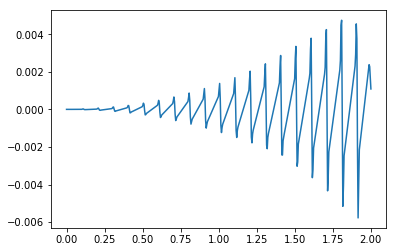
\includegraphics[width=.9\linewidth]{obipy-resources/73232f0e737f26c048822a8e09245932-2031Yqg.png}
\end{center}



\section{{\bfseries\sffamily ASSIGNED} exam3-6\hfill{}\textsc{quad:integration:mingjie:p1:2}}
\label{sec:org0798cc2}
\textbf{This is an exam. You must be present in the exam room to get credit for this problem unless you have prior permission from the instructor. You may not talk during the exam except to ask an instructor a question. By turning this in, you agree that this work is your own, and you did not get unauthorized help to complete it or provide unauthorized help to anyone else. You may not modify your exam answer after the due time without permission.}

The \(\Gamma\) function is defined by:

\(\Gamma(x) = \int_0^\infty e^{-t}t^{x-1} dt\)

It is a generalized factorial function. When the arguments to the function are integers, the following relation is true:

\(\Gamma(n + 1) = n!\)

Show that this is true for the integers from 1 to 10. You can use the \texttt{math.factorial} function.

\begin{minted}[frame=lines,fontsize=\scriptsize,linenos]{ipython}
from math import factorial

factorial(4)
\end{minted}

\begin{verbatim}
24
\end{verbatim}

\subsection{solution\hfill{}\textsc{solution}}
\label{sec:orgf52e1ce}

\begin{minted}[frame=lines,fontsize=\scriptsize,linenos]{ipython}
from math import factorial
from scipy.integrate import quad
import numpy as np

def integrand(t, x):
    return np.exp(-t) * t**(x - 1)

def Gamma(x):
    I, err = quad(integrand, 0, np.inf, args=(x, ))
    return I

for i in range(1, 11):
    print(i, Gamma(i), factorial(i - 1))
\end{minted}

1 1.0000000000000002 1
2 0.9999999999999998 1
3 2.0 2
4 6.0 6
5 24.0 24
6 120.00000000000001 120
7 720.0000000000001 720
8 5040.000000000001 5040
9 40320.0 40320
10 362879.99999999994 362880
\end{document}